\section{Introduction}

This laboratory main objective is to conceive an Alternate Current to Direct Current (AC/DC) Converter. The converter consists in a transformer and two sub-circuits, an envelope detector and a voltage rectifier circuits.\ref{Fig1: circuit}.

To build this circuit we have to maximise the merit. The merit of the work is given by:
\begin{equation}
    Merit = \dfrac{Quality}{Cost}
\end{equation}
Quality is given by the following expression:
\begin{equation}
    Quality = \dfrac{1}{Ripple(V_o)} + \dfrac{1}{Average(V_o-12)} 
\end{equation}
With $V_o$ being the Voltage output.

We also need to build the circuit as cheap as we can. Both \SI{1}{\kilo\ohm}, in a resistance, and \SI{1}{\micro\farad}, in a capacitor, cost 1 Monetary Unit (MU). Other element used is a diode which costs 0.1 MU per unit.
With this price table we can compute the cost
\begin{equation}
    Cost = N_{Diodes}*0.1+N_{Resistances}*1+N_{Capacitors}*1
\end{equation}
To achieve this we will be using a full wave rectifier for the envelope detector circuit and a resistance plus diodes in series circuit for the voltage regulator circuit.

\begin{figure}[h] 
\centering
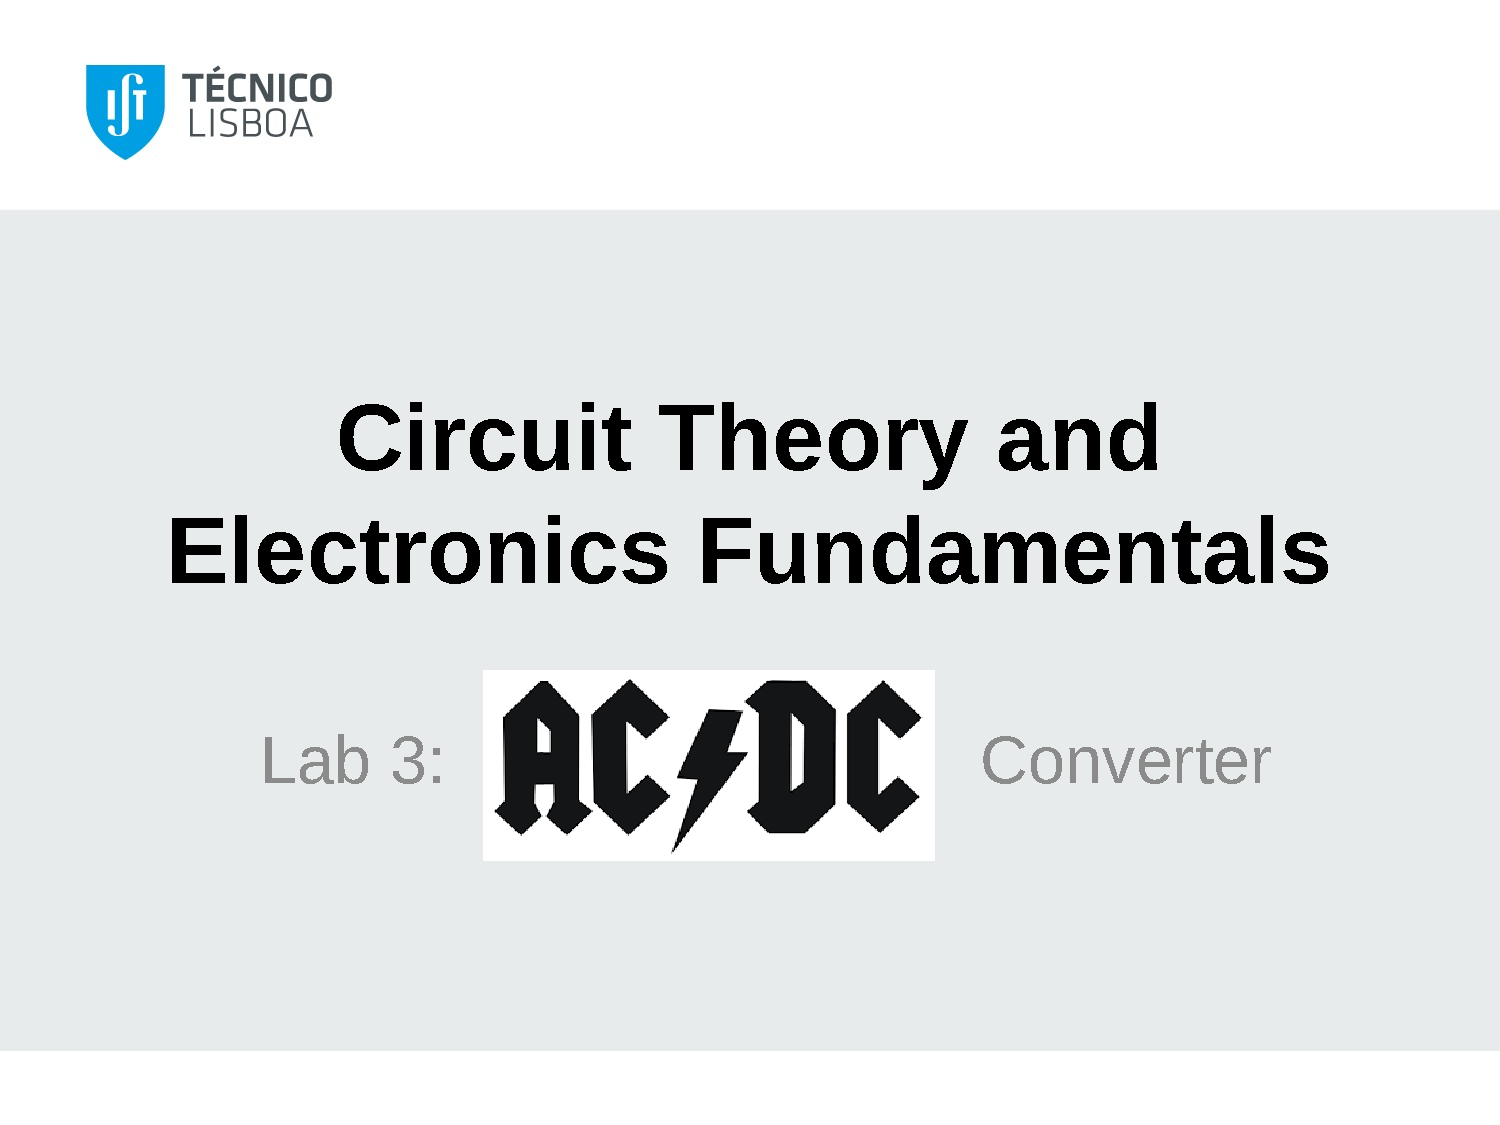
\includegraphics[width=0.6\linewidth]{t3.pdf}
\caption{Circuit Concept.}
\label{Fig1: circuit}
\end{figure}

Plots and results are shown after the \ref{sec:analysis} and \ref{sec:simulation} sections for easier comparison.
